
\chapter{Statistics and Probability}
\section{Definition of Moments}
Let $x\in\mathbb R^{n}$ is a random variable.
We write $m = E[x]\in\mathbb R^n$ for the expectation and
$M=\mathrm{Var}[x] = E[(x-m)(x-m)^T]$ for the covariance (when these quantities are defined.)

In tensor diagrams, we will use square brackets:
\[
\mathbin{\begin{tikzpicture}[baseline=(n0.base), inner sep=1pt]
   \node (n0) at (0,0) {$m=[$};
   \node [right=1em of n0] (n1) {$x]$};
   \draw (n0) -- (n1);
\end{tikzpicture}}
\quad\text{and}\quad
\mathbin{\begin{tikzpicture}[baseline=(n0.base), inner sep=1pt]
   \node (n0) at (0,0) {$M=[$};
   \node [right=1em of n0] (n1) {$(x\ominus m)$};
   \node [right=.5em of n1] (n2) {$(x\ominus m)$};
   \node [right=1em of n2] (n3) {$]$};
   \draw (n0) -- (n1);
   \draw (n2) -- (n3);
\end{tikzpicture}}
\]
We will use the circled minus, $\ominus$, to distinguish the operation from contraction edges.

We can also define the third and fourth centralized moment tensors
\[
   M_3=
   \renewcommand*{\arraystretch}{1.3}
   \begin{bmatrix}
      \vecmatvec{1em}{(x\ominus m)}{}{} \\
      \vecmatvec{1em}{(x\ominus m)}{}{} \\
      \vecmatvec{1em}{(x\ominus m)}{}{}
   \end{bmatrix}
\quad\text{and}\quad
M_4=
   \renewcommand*{\arraystretch}{1.3}
   \begin{bmatrix}
      \vecmatvec{1em}{(x\ominus m)}{}{} \\
      \vecmatvec{1em}{(x\ominus m)}{}{} \\
      \vecmatvec{1em}{(x\ominus m)}{}{} \\
      \vecmatvec{1em}{(x\ominus m)}{}{}
   \end{bmatrix}
.
\]
These are less common in introductory causes, even though the scalar third and fourth moment are common.
This is presumably because they require higher order tensors.

\section{Expectation of Linear Combinations}
General principle: The ``linearity of expectation'' lets you pull out all parts of the graph not involving $X$.
\[
   \vcenter{\hbox{
      \import{figures/}{linearityOfExpectations.pdf_tex}
   }}
\]
where $M$ is the expectation of the product of the four instances of $X$, with no dependence of the constants $A$, $B$, $C$ and $D$.
Note however that the way in which in $X$s are multiplied together matters, creating many possible raw ``fourth moments'' this way.

\subsection{Linear Forms}
The Matrix Cookbook gives the following simple expectations:
\begin{align*}
   \tag{312}
   \E[AXB+C] &= A \E[X] B + C
   &
   \renewcommand*{\arraystretch}{1.3}
   \begin{bmatrix}
      \matmul{A,X,B} \\+\, \matmul{C}
   \end{bmatrix}
   &=
   \renewcommand*{\arraystretch}{1.3}
   \begin{matrix}
      \matmul{A,[X],B} \\+\, \matmul{C}
   \end{matrix}
   %%%%%%%%%%%%%%%%%%%%%%%%%%%%%%%%%%%%%%%%
   \\
   \tag{313}
   \mathrm{Var}[Ax] &= A \mathrm{Var}[x] A^T
   &
   \renewcommand*{\arraystretch}{1.3}
   \begin{bmatrix}
      \vecmatvec{.5em}{A}{}{x} \ominus [\vecmatvec{.5em}{A}{}{x}] \\
      \vecmatvec{.5em}{A}{}{x} \ominus [\vecmatvec{.5em}{A}{}{x}]
   \end{bmatrix}
   &=
   \renewcommand*{\arraystretch}{1.3}
   \begin{bmatrix}
      \vecmatvec{.5em}{A}{}{(x\ominus m)} \\
      \vecmatvec{.5em}{A}{}{(x\ominus m)}
   \end{bmatrix}
 \\&&&=
   \vcenter{\hbox{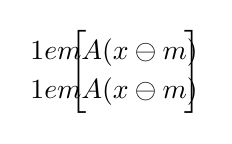
\begin{tikzpicture}[inner sep=1pt]
      \node (n1) at (0,-.25) {$\vecmatvec{1em}{A}{}{(x\ominus m)}$};
      \node (n2) at (0,.25) {$\vecmatvec{1em}{A}{}{(x\ominus m)}$};
      \node at (-.45, 0) {$\Bigg[$};
      \node at (1, 0) {$\Bigg]$};
   \end{tikzpicture}}}
 \\&&& =
   \vecmatvec{.5em}{}{A,M_2,A}{}
\end{align*}

\subsection{Quadratic Forms}
We often prefer to write expectations in terms of the simple centered moments, which we can do by pulling out the mean:
\begin{align*}
   \E[x^T A x]
   &= \mathrm{Tr}(A \Sigma) + \mu^T A \mu
   &
   [\vecmatvec{.5em}{x}{A}{x}]
   &=
   \left[
      \begin{cases}
      \vecmatvec{.5em}{(x\ominus \mu)}{A}{(x \ominus\mu)}
      + \vecmatvec{.5em}{\mu}{A}{\mu}
      \\
      \vecmatvec{.5em}{(x\ominus \mu)}{A}{x}
      + \vecmatvec{.5em}{x}{A}{(x \ominus\mu)}
   \end{cases}
   \right]
   \\
   &&&=
   \mathbin{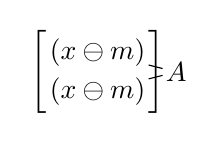
\begin{tikzpicture}[inner sep=1pt]
      \node (n1) at (0,-.25) {$(x\ominus m)$};
      \node (n2) at (0,.25) {$(x\ominus m)$};
      \node at (-.75, 0) {$\Bigg[$};
      \node at (.75, 0) {$\Bigg]$};
      \node (A) at (1, 0) {$A$};
      \draw (n1) -- (A);
      \draw (n2) -- (A);
   \end{tikzpicture}}
   +
   \vecmatvec{.5em}{\mu}{A}{\mu}
   \\
   &&&=
   \trace{\Sigma,A}2
   +
   \vecmatvec{.5em}{\mu}{A}{\mu}
\end{align*}

\subsection{Cubic Forms}
TODO

\section{Weighted Scalar Variable}
Let $y=w^T x$, and let $m=E[y]$, then
\begin{align*}
   \E[y] &= m = w^T \mu
   \\
   \E[(y\ominus m)^2] &= \vecmatvec{.5em}{w}{M_2}{w}
   \\
   \E[(y\ominus m)^3] &=
   \mathbin{\begin{tikzpicture}[baseline=(a0.base), inner sep=1pt]
      \node (a0) {$M_3$};
      \node[above=.3em of a0] (n0) {$w$};
      \node[right=.3em of a0] (n1) {$w$};
      \node[left=.3em of a0] (n3) {$w$};
      \draw (a0.north) -- (n0);
      \draw (a0.east) -- (n1);
      \draw (a0.west) -- (n3);
   \end{tikzpicture}}
   \\
   \E[(y\ominus m)^4] &=
   \mathbin{\begin{tikzpicture}[baseline=(a0.base), inner sep=1pt]
      \node (a0) {$M_4$};
      \node[above=.3em of a0] (n0) {$w$};
      \node[right=.3em of a0] (n1) {$w$};
      \node[below=.3em of a0] (n2) {$w$};
      \node[left=.3em of a0] (n3) {$w$};
      \draw (a0.north) -- (n0);
      \draw (a0.east) -- (n1);
      \draw (a0.south) -- (n2);
      \draw (a0.west) -- (n3);
   \end{tikzpicture}}
\end{align*}
For specific distributions, like $x$ Gaussian, we can often reduce the moment tensors further.
Khintchine's inequality also gives a way to bound all of these in terms of $E[(y-m)^2]$.


\section{Gaussian Moments}
\subsection{Gaussian Integration by Parts}
If $X$ is a tensor with Gaussian entries, zero mean, and some covariance,
% General principle for Gaussian expectations.
Stein's lemma gives the following very general equation, for any differentiable function $f$:
\[
   \vcenter{\hbox{
      \import{figures/}{steins.pdf_tex}
   }}
\]
Combined with the tensor chain rule from chapter~\ref{chapter:functions}, this can be a very powerful way to evaluate many hard expectations.

\subsection{Mean and covariance of linear forms}
TODO
\subsection{Mean and variance of square forms}
TODO
\subsection{Cubic forms}
TODO
\subsection{Mean of Quartic Forms}
TODO


